\documentclass{labo}
\usepackage[utf8x]{inputenc}

\usepackage[english]{babel}
\usepackage[T1]{fontenc}

\usepackage{graphicx}
\usepackage{amssymb}
\usepackage{amsmath}
\usepackage{siunitx}
\usepackage{wasysym} %smiley
\usepackage{textcomp}
% \usepackage{minted}
\usepackage[long]{datetime}
\usepackage{gensymb} % \ohm, celsius
\usepackage{framed}
\usepackage{pdfpages}
\usepackage{paralist}

\usepackage{mathastext} % math as standfard text : units are respecting typography conventions.
\usepackage{fancyhdr} %en-tête
\usepackage{qrcode}
\usepackage{pgfplots} %for latex grid
\usepackage{fontawesome}
\usepackage{charter}
\usepackage{subfig}

\usepackage{minted}

%%%%%%%%%%%%faHandPeaceO
% Tables
%%%%%%%%%%%%
\usepackage{dcolumn}
\newcolumntype{.}{D{.}{.}{2}}
\usepackage{booktabs}
\renewcommand{\arraystretch}{1.1} % Opens up the table a tad
\usepackage{multicol}
\usepackage{multirow}

\langexam{frenchb}

\correction{false}
%\correction{true}

\author{}


%% fancy header & foot
\pagestyle{fancy}
\lhead{[4EISA] Image Processing\\ LAB 4 \ifthenelse{\boolean{corrige}}{~-- correction}{}}
\rhead{v1.0.0\\ page \thepage}
\cfoot{}
%%

\pdfinfo{
/Author ()
/Title (4EISA Image Processing, lab 4)
/ModDate (D:\pdfdate)
}

\hypersetup{
pdftitle={LAB 4 [4EISA] Image Processing},
pdfauthor={},
pdfsubject={}
}

\newcommand{\numpy}{\texttt{NumPy} }
\newcommand{\opencv}{\texttt{OpenCV} }

\setminted[python]{
frame=lines,
framesep=2mm,
% baselinestretch=1.2,
fontsize=\small,
linenos
}

\begin{document}

\tptitle{}{Image Processing -- Session 4\\}

This session is devoted to the assignment you will need to handle by the date specified on Claco.
You can choose any subject within the following list or make up your own.
For each challenge, there are several levels; the higher the level reached, the better.


\section*{Counting fingers and recognising gestures}
With a single hand on screen, read the instructions it might be sending your way.

\begin{description}
	\item[Level 1] Detect and interpret the amount of fingers on screen.
	\item[Level 2] Detect and interpret the position of the fingers \faHandPeaceO \faHandSpockO \faHandScissorsO
	\item[Level 3] Detect and interpret the movement of the hand or fingers.
	\item[Level Bonus] Play Rock-paper-scissors with the computer.
\end{description}


\section*{Cheat the Ishihara Test}
The Ishihara test purpose is to diagnose variations of colour blindness or deficiencies\footnote{\href{https://en.wikipedia.org/wiki/Ishihara\_test}{Ishihara test on Wikipedia}, \href{http://daltonien.free.fr/daltonien/article.php3?id_article=6}{complete test here}.}.
Your aim is to cheat the test using computer vision. Your program should be able to analyse various plates and detect its features.

\begin{center}
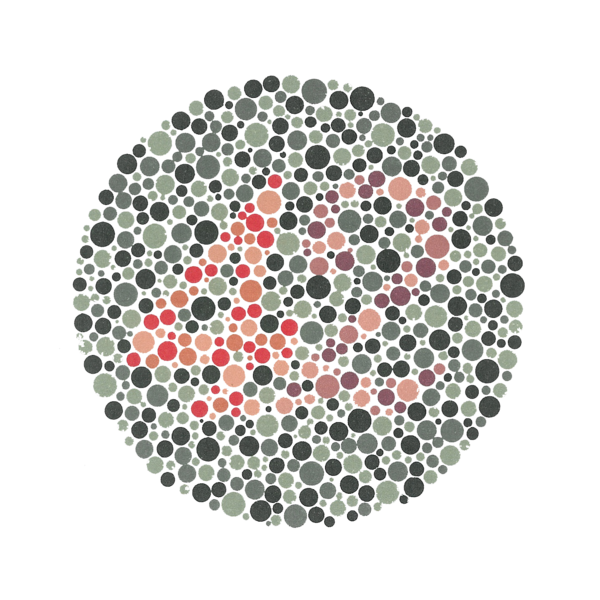
\includegraphics[width=.4\textwidth]{Ishihara_23.PNG}
\end{center}

\begin{description}
	\item[Level 1] Highlight the colours.
	\item[Level 2] Change the colour scheme to black\&white to highlight the number.
	\item[Level 3] Make it working with a live video feed from the camera and superimpose the previous result on the actual image.
	\item[Level 4] Recognise and translate the number from the test.
\end{description}


\section*{Make up your own challenge}
You have a great idea about a challenge involving computer vision and \opencv? Great, talk about it with a teacher to set the specifications and make sure you are within the expectations of the course.


\section*{Evaluation}
You should hand the following items in your submission:
\begin{itemize}
	\item A report
	\item Your code
	\item A demonstration
\end{itemize}

Your report should be no longer than four pages long and have at least the following key points:
\begin{itemize}
	\item Description of the context/situation chosen and expected results.
	\item Identification of the key challenges of the problem.
	\item Strategy to tackle the aforementioned challenges, how to implement a solution.
	\item Results and discussion of their quality.
	\item How to take it further.
\end{itemize}

Your code can be either handed in an archive or through GitHub and the like.
The demonstration should be a recording of your screen showing the processing in action\footnote{Checkout \href{https://obsproject.com/}{OBS} to record your screen.}. Upload it on a video hosting platform and add a link in your report, rather than uploading it directly on Claco.



\end{document}
